\documentclass{article}
\usepackage{amsmath}
\usepackage{amssymb}
\usepackage[usenames, dvipsnames]{color}
\usepackage{gensymb}
\usepackage{hyperref}
\usepackage{tikz}
\usepackage{geometry}
\usepackage[normalem]{ulem}

\title{\vspace{-3em}The Sky-Diving Trainhopper\vspace{-3em}}

\geometry{letterpaper, portrait, margin=0.5in}

\definecolor{myred1}{RGB}{255, 0, 0}
\definecolor{myyellow1}{RGB}{255, 255, 219}
\definecolor{mygreen1}{RGB}{0, 255, 0}
\definecolor{mygreen2}{RGB}{0, 126, 0}
\definecolor{myblue1}{RGB}{0, 0, 255}

\begin{document}

\fontsize{14}{16}\selectfont

% center the title
\maketitle

Om is a skydiving trainhopper. A freighter steam locomotive is going downhill on a straight track that makes an angle of elevation with the ground of $\theta=37.13\degree$. Unfortunately, the train's engine has failed and the wheels are sliding down the frictionless tracks. Luckily, the train has a backup jet propulsion engine. The horizontal distance the hill comprises is 300 meters.

\section{How fast is Om dying?}
[riley insert yap]

\section{How fast is that engine going?}
Given the mass of the train is $m=550000$ kg and the time $t$ you found from the previous problem. You are finding the Work that the jet propulsion engine needs to do on the train for it to reach the bottom of the hill just in time to catch Om at the front of the engine.

\section{Part III}

\pagebreak

\section{Answer}

\subsection{How fast is Om dying?}

\subsection{How fast is that engine going?}

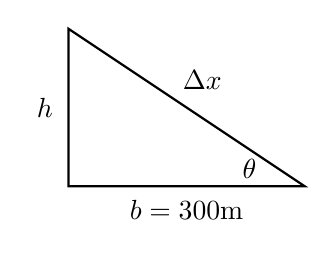
\begin{tikzpicture}
    \draw [thick] (0,0) -- (3,0) -- (0,2) -- cycle;
    \draw (1.5,-0.3) node {$b=300$m};
    \draw (-0.3,1) node {$h$};
    \draw (1.7,1.35) node {$\Delta x$};
    \draw (2.3,0.22) node {$\theta$};
\end{tikzpicture}

\begin{align*}
    h=b\tan\theta 
    \Longrightarrow h=(300\text{m})\tan(37.13\degree) \approx 227.135\text{m}
    \\
    \Delta x=b\sec\theta
    \Longrightarrow \Delta x=(300\text{m})\sec(37.13\degree) \approx 376.285\text{m}
\end{align*}
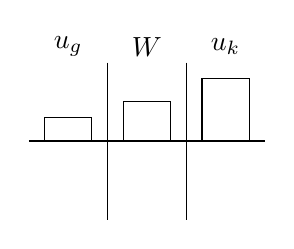
\begin{tikzpicture}
    \draw [thick] (0,0) -- (3,0);
    \draw (1,1) -- (1,-1);
    \draw (2,1) -- (2,-1);
    \draw (0.5,1.2) node {$u_g$};
    \draw (1.5,1.2) node {$W$};
    \draw (2.5,1.2) node {$u_k$};
    \draw[rectangle, draw=black] (0.2,0) rectangle (0.8,0.3);
    \draw[rectangle, draw=black] (1.2,0) rectangle (1.8,0.5);
    \draw[rectangle, draw=black] (2.2,0) rectangle (2.8,0.8);
\end{tikzpicture}

\begin{align*}
    u_k=\frac{1}{2}mv^2 \quad u_g=mgh \\
    \Longrightarrow W=\frac{1}{2}mv^2-mgh \\
    v_f=v_0+at 
    \quad x_f=x_0+v_0t+at^2 \Longrightarrow x_f=\frac{1}{2}at^2 \Longrightarrow \frac{2x_f}{t}=at \\
    v_f=\frac{2x_f}{t} \\
    \Longrightarrow W=m(\frac{1}{2}\biggr(\frac{2x_f}{t}\biggr)^2-gh) \\
    \Longrightarrow W=m(2\biggr(\frac{x_f}{t}\biggr)^2-gh)
    \Longrightarrow W=(550000\text{kg})(2\biggr(\frac{376.285\text{m}}{t}\biggr)^2-\biggr(9.8\frac{\text{m}}{\text{s}^2}\biggr)(227.135\text{m}))
\end{align*}
Riley add the time and do the solving

\end{document}
